\documentclass{article} 
\usepackage{tikz}
\usetikzlibrary{trees}
\begin{document}
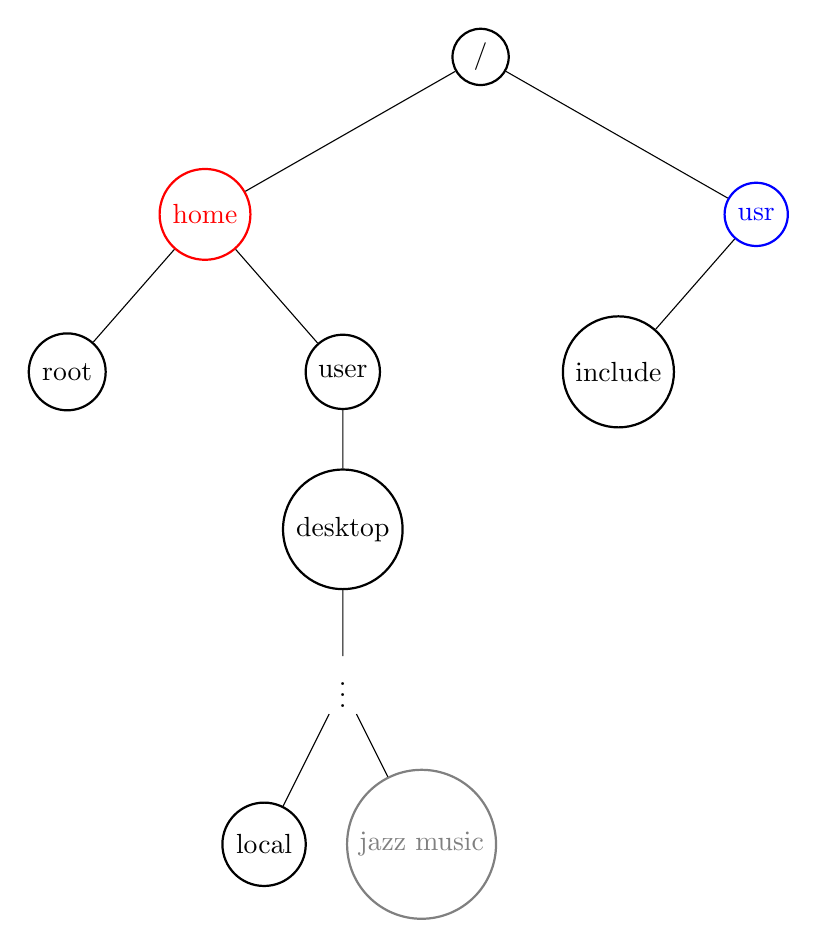
\begin{tikzpicture}[level distance=2cm,
  level 1/.style={sibling distance=7cm},
  level 2/.style={sibling distance=3.5cm},
  level 3/.style={sibling distance=2cm}]

%La forma del nodo aumenta automaticamente dependiendo del contenido
  \node [circle,draw,thick] {/}
    child { node [circle,red,draw,thick] {home}
      		child {node [circle,draw,thick] {root}}
      		child {node [circle,draw,thick] {user}
      		child {node [circle,draw,thick] {desktop}%Nodo desbalanceado
			child {node {$\vdots$}%Muchos nodos mas abajo
				child{node [circle,draw,thick] {local}}
				child{node [circle,black!50,draw,thick] {jazz music}}
}}}
    }
    child {node [circle,blue,draw,thick] {usr}
    		child {node [circle,draw,thick] {include}}
    		child[missing] {node [circle,draw,thick] {}}%Para crear un nodo vacio 
    };





\end{tikzpicture}
\end{document}
